\documentclass[times, utf8, zavrsni, numeric]{fer}
\usepackage{booktabs}
\usepackage{pdfpages}
\usepackage{float}
\usepackage{hyperref}
\usepackage{listings}
\usepackage{xcolor}
\usepackage{amsmath}
\usepackage[clean]{svg}

\definecolor{codegreen}{rgb}{0,0.4,0}
\definecolor{commentgreen}{rgb}{0, 0.6, 0}
\definecolor{codegray}{rgb}{0.5,0.5,0.5}
\definecolor{codeorange}{rgb}{1.00,0.33,0.00}
\definecolor{backcolour}{rgb}{0.97,0.97,1.00}

\lstdefinestyle{mystyle}{
    backgroundcolor=\color{backcolour},   
    commentstyle=\color{commentgreen},
    keywordstyle=\color{codeorange},
    numberstyle=\tiny\color{codegray},
    stringstyle=\color{codegreen},
    basicstyle=\ttfamily\footnotesize,
    breakatwhitespace=false,         
    breaklines=true,                 
    captionpos=b,                    
    keepspaces=true,                 
    numbers=left,                    
    numbersep=5pt,                  
    showspaces=false,                
    showstringspaces=false,
    showtabs=false,                  
    tabsize=2
}

\lstdefinelanguage{docker-compose-2}{
  keywords={version, volumes, services},
  keywordstyle=\color{codegreen},
  keywords=[2]{image, environment, ports, container_name, ports, links, build},
  keywordstyle=[2]\color{codeorange},
  identifierstyle=\color{black},
  sensitive=false,
  comment=[l]{\#},
  commentstyle=\color{purple}\ttfamily,
  stringstyle=\color{red}\ttfamily,
  morestring=[b]',
  morestring=[b]"
}

\lstset{style=mystyle}

\tolerance=1
\emergencystretch=\maxdimen
\hyphenpenalty=10000
\hbadness=10000

\renewcommand{\chapterautorefname}{Poglavlje }
\renewcommand{\sectionautorefname}{Odjeljak }
\renewcommand{\subsectionautorefname}{Pododjeljak }
\renewcommand{\lstlistingname}{Kodni isječak}

\begin{document}

\thesisnumber{660}

\title{Sustav za označavanje tekstualnog sadržaja navođeno aktivnim učenjem}

\author{Franjo Mindek}

\maketitle  

% Ispis stranice s napomenom o umetanju izvornika rada. Uklonite naredbu \izvornik ako želite izbaciti tu stranicu.
% \izvornik
\includepdf[pages=-]{zadatak.pdf}

% Dodavanje zahvale ili prazne stranice. Ako ne želite dodati zahvalu, naredbu ostavite radi prazne stranice.
\zahvala{}

\tableofcontents

% TOC za završni
% Uvod
% Označavanje podataka (tu pišeš o važnosti specijalnih datasetova, data quality, etc.)
% Aktivno učenje (tu popišeš mehanizme iz literature)
% Problem
% Rezultati
% Zaključak
% cilj 32 stranice do 10 eksperimentalni dio

\chapter{Uvod}
Zbog potrebe rješavanja UI\footnote{UI - umjetna inteligencija}-potpunih problema sve se više susrećemo s raznim primjenama strojnog učenja.
Ipak, zbog ulazno-izlazne povezanosti podataka i rezultata modela strojnog učenja nužno je imati kvalitetan skup podataka.

Većina problema umjetne inteligencije rješava se treniranjem modela nad indiskriminativno skupljenim podatcima koji su često označeni za preopćenitu ili nama krivo specifičnu svrhu, nisu potpuni i sadrže netočne informacije. Rezultat toga je potreba za ogromnim skupovima podataka varirajuće kvalitete kako bi se približili željenoj efikasnošću modela \citep{baliga1997learning}. Uspjeh samog modela zasniva se na kvalitetnom skupu podataka koji efikasno razapinje prostor problema, što modelu omogućuje pouzdane i precizne odgovore \citep{jain2020overview}.

Cilj aktivnog učenja je povećati uzorkovanu učinkovitost postupka utreniravanja modela minimizirajući broj podataka i maksimizirajući dobit traženog informacijskog svojstva \citep{settles2009active}.
Tim postupkom smanjujemo trošak i vrijeme stvaranja \citep{baldridge2009well} te veličinu skupa podataka dok istovremeno povećavamo i preciznost modela.

U ovom završnom radu koristeći javno dostupne alate, implementirat ćemo sustav za označavanje tekstualnog sadržaja navođeno aktivnim učenjem.
Označivačima podataka bit će ponuđeno web sučelje koje će ih uvesti u postupak označavanje te će im zadavati uzorke visoke informacijske dobiti za odabrani model.

\chapter{Označavanje podataka}

Označavanje podataka je jedan od početnih koraka u procesu stvaranju modela strojnog učenja te ga svrstavamo u razinu pretprocesiranja. 
Definiramo ga kao proces prepoznavanja neobrađenih podataka (slika, tekst, video\dots) koji se onda pomoću jedne ili više oznaka opisuju u kontekstu modela, što dozvoljava modelu strojnog učenja da može stvarati točna predviđanja.

Označavanje podataka često je najsporiji i najvažniji dio modeliranja modela strojnog učenja. U prosjeku više od 80\% ukupnog vremena modeliranja umjetne inteligencije potroši se na rad s podacima \citep{cognilytica2019}. Vremenska neefikasnost označavanja podataka dovela je do potrebe razvoja modela umjetne inteligencije koji pomažu u procesu označavanja podataka. Jedan primjer takve umjetne inteligencije je aktivno učenje čiji ćemo utjecaj na označavanje podataka obraditi u \autoref{chap:aktivno_ucenje}.

\begin{figure}[h]
\centering
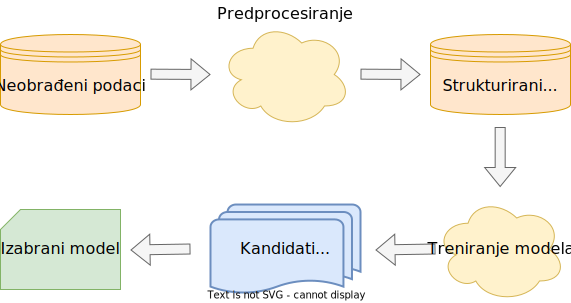
\includegraphics[width=\textwidth]{pictures/proces_strojnog_ucenja.png}
\caption{Pojednostavljeni dijagram stvaranja modela strojnog učenja.}
\label{proces_strojnog_ucenja}
\end{figure}

\section{Strojno učenje i podatci}

% Strojno učenje je proces koji započinje obradom podataka, a završava stvaranjem modela strojnog učenja.
Problem s kojim se danas u svijetu često susrećemo jest to da imamo pristup obilju podataka, danas skupovi podataka često se broje u milijunima redaka. U susretu s takvom količinom podataka čovjeku je prezahtjevan posao da iz njih izvući sve međusobne skrivene povezanosti. Upravo iz potrebe iskorištavanja tog informacijskog potencijala razvijali su se sustavi koji na temelju podatak mogu učiti, a po završetku učenja nuditi korisna ponašanja. Uspješan primjer takvih sustava je umjetna inteligencija, gdje nam je posebno zanimljiva grana strojnog učenja zbog njene povezanost s podacima.
% Da bismo razumjeli zašto su nam potrebni dobri podatci i njihovo ispravno označavanje krenut ćemo od njihove svrhe u procesu strojnog učenja. Svrha skupa podataka je izvući korisne informacije i povezanosti koje je običnom čovjeku teško uočiti. 
% Strojno učenje možemo opisati sljedećom definicijom. 

Strojno učenje je programiranje računala na način da optimiziraju neki kriterij uspješnosti temeljem podatkovnih primjera ili prethodnog iskustva. Raspolažemo modelom koji je definiran do na neke parametre, a učenje se svodi na izvođenje algoritma koji optimizira parametre modela na temelju podataka ili prethodnog iskustva \citep{alpaydin2020introduction}.

Iz prethodnih definicija možemo uočiti povezanost između strojnog učenja i skupa podataka. Odgovor ili rješenje problema kojeg zahtijevamo od strojnog učenja je izlaz, ali taj izlaz možemo dobiti samo temeljem ulaza. Ako smo odabrali dobar skup podataka vrlo vjerojatno doći ćemo do traženog rješenja problema (osim ako su podaci prekomplicirani za izabrani model), no ako je naš skup podataka na bilo koji način iskrivljen ta iskrivljenost će se propagirati i na izlaze, što dovodi do krivih spoznaja.

Općenito se u strojnom učenjem susrećemo s dva tipa podataka, to su numerički ili kategorički podatci. Numeričke podatke predstavljaju brojevi nad kojima možemo vršiti računske operacije. To može biti visina čovjeka, cijena dionica, količina prodanih artikala i slično. Kategorički podatci su podatci podijeljeni u kategorije. Dijelimo ih na 2 vrste kategoričkih varijabli, nominalne i ordinalne. Razlikuju se po tome što nominalne varijable nemaju definiran poredak unutar kategorija. Primjer nominalne kategorije jest kada trebamo kategorizirati životinje sa slike, a dane su nam opcije "pas", "mačka" i "krava". Nemoguće je uspostaviti značenje usporedbe "krava" > "mačka". S druge strane ordinalne kategorije često možemo susresti u anketama zadovoljstva korisnika. Ako su korisniku ponuđene opcije "potpuno zadovoljan", "skoro potpuno zadovoljan", "jako zadovoljan"\dots podatke možemo lako staviti u poredak. Ono što je zajedničko nad oba kategorička primjera jest da nad njima ne možemo raditi aritmetiku. 

\subsection{Paradigme strojnog učenja i strukturiranost skupa podataka}

U pravilu strojno učenje možemo podijeliti u tri paradigme koje se između ostaloga razlikuju po izvoru informacija pomoću kojih se treniraju. Ovisno o izabranoj paradigmi i samoj namjeni modela drukčije ćemo pristupati procesu strukturiranja podataka.

\subsubsection{Nadzirano učenje}

Cilj nadziranog učenja je naučiti model kako ulaz preslikavati na izlaz. Definirano je korištenjem označenih skupova podataka koji sadrže informacije o ulazu i značajkama tog ulaza, to jest izlazu svakog uzorka. Ti skupovi podataka treniraju i \glqq nadziru\grqq{} algoritam u procesu klasifikacije ili regresije. To jest, na temelju poznatih rješenja predviđamo rješenje problema, ili u smislu podataka, predviđamo izlaz za nove, neoznačene podatke na temelju označenih podatka. 

Naziv nadziranog učenja dolazi iz profesor-student odnosa tijekom procesa treniranja modela. Profesor usmjerava studenta iz kojih materijala učiti, a po završetku učenja student se ocjenjuje. Ako je student točan prolazi bez ispravljanja, ako je pak netočan, profesor ispravlja studenta i navodi ga da uči na temelju svojih pogrešaka.
% Podatci se nadziru tako što model koristeći označene podatke (koje nije koristio tijekom treniranja)  može mjeriti svoju preciznost.

\begin{figure}[H]
    \centering
    \includegraphics[width=0.8\textwidth]{pictures/nadzirano_ucenje.jpg}
    \caption{Ilustracija odnosa tijekom modeliranja modela nadziranog učenja. \citep{nadzirano_slika}}
    \label{nadzirano_ucenje_slika}
\end{figure}

Klasifikacija označava da radimo s izlazom koji je kategorička varijabla, što znači da naš izlaz treba poprimiti vrijednost jedne od preddefiniranih kategorija. Na primjeru poštanskog sandučića, dolaznu poštu možemo kategorizirati na \textit{spam} i normalnu poštu.

Regresija ipak označava da radimo s izlazom brojčane vrijednosti. Cilj regresije je riješiti problem otkrivanja veza zavisnih i nezavisnih varijabli. Primjer toga može biti da imamo tvrtku koja svake godine ulaže u razne vrste marketinga. Sada na primjeru povijesnih podataka želi predvidjeti prodaju nove marketinške kampanje.

\begin{figure}[H]
    \centering
    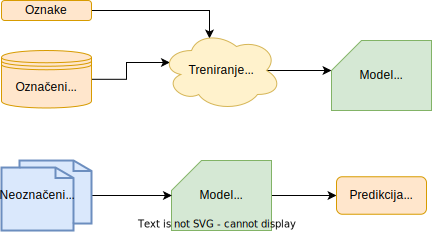
\includegraphics[width=\textwidth]{pictures/nadzirano.png}
    \caption{Pojednostavljeni dijagram faze učenja i iskorištavanja modela nadziranog učenja}
    \label{nadzirano_dijagram}
\end{figure}

\subsubsection{Nenadzirano učenje}

Nenadzirano učenje se koristi kada skup podataka nije označen, to jest kada nisu definirani izlazi ulaza. Koristi se kada je takve podatke potrebno analizirati i grupirati. Cilj je da algoritam otkrije skrivene uzorke ponavljanja u podacima bez potrebe ljudskog nadzora. U postupke nadziranog učenja spadaju grupiranje, otkrivanje stršećih/novih vrijednosti, otkrivanju povezanosti i smanjenje dimenzionalnosti.

Cilj grupiranja jest da podatke na temelju sličnost razdijeli u određeni broj kategorija. Taj broj kategorija možemo biti unaprijed određen, ili dinamički izračunat od strane algoritma.

Postupak otkrivanja stršećih/novih vrijednosti pokušava naći podatke unutar skupa podataka koji su se po nekom određenom kriteriju dovoljno razlikuju. Ti podatci često predstavljaju pogreške u podacima ili neke nove spoznaje, zbog čega ih i želimo otkriti.

\begin{figure}[H]
    \centering
    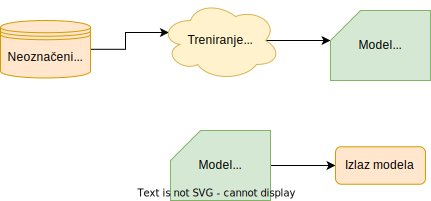
\includegraphics[width=\textwidth]{pictures/nenadzirano.png}
    \caption{Pojednostavljeni dijagram faze učenja i iskorištavanja modela nenadziranog učenja}
    \label{nenadzirano_dijagram}
\end{figure}

\subsubsection{Podržano učenje}

Podržano/ojačano učenje predstavlja dio strojnog učenja koje se bavi optimizacijom ponašanja gdje je cilj učenje optimalne strategije na temelju pokušaja s odgođenom nagradom. Definirano je agentom, okolinom i akcijama koje agent može raditi. Agent na temelju informacija iz okoline obavlja akcije za koje je onda nagrađen ili kažnjen, a njegova je zadaća otkriti strategiju tako da maksimizira nagrade koje dobiva \textit{na duge staze}.

\begin{figure}[H]
    \centering
    
\includegraphics[width=\textwidth]{pictures/podrzano.png}
    \caption{Pojednostavljeni dijagram podržanog učenja}
    \label{podrzano_dijagram}
\end{figure}


% \begin{figure}[H]
% \centering
% \includegraphics[width=\textwidth]{pictures/3paradigme.jpg}
% \caption{Vizualna reprezentacija 3 paradigme strojnog učenja. \citep{3paradigme}}
% \label{3paradigme}
% \end{figure}


\section{Karakteristike dobrog skupa podataka}

Karakteristike modela strojnog učenja, a time i skupova podataka nad kojima se trenira uvelike ovise o namjeni umjetne inteligencije. Svejedno možemo opisati određena svojstva koja su uvijek poželjna unutar skupa podataka neovisno o njihovoj primjeni.

\begin{enumerate}
    \item Potpunost - pretpostavka je da u skupu podataka ne postoje prazne \glqqćelije\grqq{}. Svaki uzorak unutar skupa podataka mora sadržavati informacije o svim traženim oznakama. Neispravne uzorke treba nadopuniti informacijama ili izbrisati iz skupa podataka. \citep{baliga1997learning}
    \item Objedinjenost - potrebno je pokriti cijelo područje problema koje se rješava. Primjer, model koji predviđa emocije preko slike lica osobe mora u svom skupu podataka sadržavati slike lica ljudi iz raznih kultura i različitih fizičkih karakteristika. Kako različite kulture drukčije iskazuju emocije, a i postoje fizičke razlike u strukturama lica, bez dovoljne objedinjenosti model ne bi zadovoljavao svojstvo generalizacije. \citep{johnson2019survey} \citep{ali2013classification}
    \item Relevantnost - podatci ne bi trebali pokrivati područje izvan problema. Pokrivanjem područja koji nisu dio našeg problema smanjuje se preciznost unutar područja problema. Kod skupova podataka sakupljenih s vanjskih izvora potrebno je filtrirati samo nama korisne informacije. Često je posljedica nerazumijevanja svojstva objedinjenosti podataka.
    \item Ortogonalnost - prostor problema koji opisujemo trebamo opisati sa što manje ponavljanja između uzoraka. \citep{alelyani2011effect} \citep{johnson2019survey} \citep{ali2013classification}
    \item Konzistentnost - kriterij opisivanja uzoraka skupa podataka mora ostati konzistentan. S potrebom ogromnih skupova podataka od više desetaka tisuća do nekoliko milijuna uzoraka rijetko će sve uzorke opisati jedna osoba. U takvim slučajevima s više označivača podatci svejedno moraju ostati konzistentno opisani.
    \item Ispravnost - po principu \glqq\textit{garbage in, garbage out}\grqq, neispravni podatci skupa podataka dovode do neispravnih rezultata modela. Problem je više izražen kada radimo s podacima subjektivne prirode. \citep{baliga1997learning}
    \item Suvremenost - podatci moraju opisivati trenutno stanje problema koji se opisuje. Primjer, model koji predviđa rezultat sportskog natjecanja treba biti upoznat s trenutnim stanjem suparničkih timova. U protivnom, on ne ispunjava svoju svrhu. \citep{karatas2020increasing}
\end{enumerate}

Upravo zbog potreba zadovoljavanja što više korisnih svojstava skupova podataka dovelo je do razvoja mnogih internih i javno dostupnih sustava označavanja podataka te razvoja UI sa svrhom ubrzanja i povećanja preciznosti tog procesa. \citep{cognilytica2019}

\section{Alati za označavanje podataka}

Zbog porasta veličine skupova podataka sustavi za označavanje podataka postali su nužni dio tehnologije strojnog učenja. Njihova korist može biti od bržeg označavanja do veće kvalitete i konzistentnosti označavanja podataka.

Alati omogućuju označavanje podataka pomoću lako upotrebljivih grafičkih sučelja koji proces označavanja rastavljaju na manje podzadatke. Prednost rastavljanja zadataka na podjedinice je to što određene podzadatke koje modeli strojnog učenja obavljaju velikom preciznošću možemo automatizirati te ljudima prepustiti rad nad podzadacima koje modeli još nišu savladali.

Također rastava posla na podzadatke omogućuje lakše praćenje, mjerenje i analizu posla koja dovodi do veće kvalitete označavanja podataka. Segmentacijom posla provjeru podataka možemo ostaviti osobama nadležnim za osiguravanje kvalitete pojedinog segmenta procesa.

U ovisnosti o podacima koje koristimo bitno je uzeti prikladan alat za označavanje podataka. Alati se razlikuju po funkcionalnostima administrativnog sučelja, pregledu informacija pomoću statističke analize, podržanim vrstama podataka (tekst, slika, zvuk, video\dots) i podržanim vrstama označavanja podataka (klasifikacija, označavanje sekvence\dots).

Zbog specifičnih potreba problema modeliranja strojnog učenja većina velikih poduzeća okreće se prema internom rješenju problema alata ili rjeđe profesionalnim vanjskim alatima \citep{cognilytica2019}.
Uslijed potrebe stvaranja sustava za označavanje tekstualnog sadržaja opisat ćemo dva javno dostupa alata koji pružaju web sučelje i zadovoljavaju specifičnosti zadanog problema.

\subsection{Label Studio}

Label Studio je sustav za označavanje otvorenog izvora koje integrira grafičko sučelje kroz cijeli proces označavanja. 
Omogućuje označavanje tekstualnog, slikovnog, audio, video i vremenskog sadržaja (te hibridnih oblika), podržavajući pri tome velik izbor predefiniranih predložaka pravila i sučelja označavanja podataka. U slučaju da ne sadrži predložak željene vrste označavanja podataka nudi mogućnost lakog stvaranja vlastitih pravila i sučelja. Isto tako nudi i bogate funkcionalnosti filtriranja i sortiranja već učitanih podataka, što olakšava snalaženje na velikim projektima.
Podupire organizaciju i rad na više projekata odjednom te podržava rad više korisnika istovremeno što ga činim pogodnim za rad u timovima.

Također dolazi uz gotove Docker slike\footnote{Docker slika je \textit{read-only} predložak koji sadržava instrukcije potrebne za pokretanje Docker kontejnera, tj. virtualnog okruženja potrebnog za rad programa} te predloške potrebne za pokretanje programa na popularnijim servisima u oblaku što omogućava lagano pokretanje timsko orijentiranog projekta označavanja podataka.

Ipak, problem Label Studia je to što većinu administrativnih mogućnosti skriva iza verzije za poduzetnike koja nije otvorenog izvora i zahtijeva kupovanje programa. Najveći propust je to što su svi sudionici projekta ujedno i administratori projekta, što znači da bilo koji označivač podataka može izbrisati sve podatke projekata koje označuje.
U slučaju da želimo imati raznolike uloge ovisno o zadatku i ovlastima korisnika to nije moguće ostvariti bez vlastite implementacije. \citep{label_studio_docs} \citep{label_studio_github}

\begin{figure}[H]
\centering
\includegraphics[width=\textwidth]{pictures/label_studio_types.png}
\caption{Label Studio pokušava biti \glqq{}all-in-one\grqq{} rješenje sustava označavanja podataka.}
\label{label_studio_types}
\end{figure}

\subsection{Doccano}

Doccano je također sustav za označavanje podataka otvorenog izvora koji integrira grafičko sučelje u proces označavanja podataka.
Za razliku od Label Studia, Doccano se usredotočio na označavanje tekstualnog sadržaja gdje podržava klasifikaciju, označavanje sekvenci i označavanje sekvencijskih odnosa.
Za razliku od Label Studia nema integrirano definiranje novih pravila i sučelja označavanja podataka što znači u slučaju potrebe drukčijeg načina označavanja podataka potrebno ga je implementirati u samom kodu Doccana.
Nadalje nudi puno slabiju mogućnost filtriranja i sortiranja podataka, što znači da je strukturiranost podataka koji se učitavaju u Doccano bitna.

Također omogućava rad na više projekata odjednom i istodoban rad korisnika u timskim projektima.
Za razliku od Label Studia sadrži potpuno administrativno sučelje i sposobnost dodjeljivanja prava po ulogama, što omogućava puno veću sigurnost projekta nego kod Label Studia. 

Isto dolazi uz vlastite Docker slike i predloške potrebne za pokretanje na servisima u oblaku, čime se omogućuje lagano započinjanje procesa označavanja podataka tekstualnog sadržaja. \citep{doccano_docs} \citep{doccano_github}

Kako je Doccano projekt započet samostalno od strane Hiroki Nakayama, dok iza Label Studia stoji grupa Heartex, Doccano je projekt manje dozrelosti nego Label Studio.

\begin{figure}[H]
\centering
\includegraphics[width=\textwidth]{pictures/doccano_types.png}
\caption{Doccano se primarno usredotočio na označavanje podataka tekstualnog sadržaja.}
\label{doccano_types}
\end{figure}

\subsection{Izbor alata}
\label{subs:izbor_alata}

Implementaciju alata za označavanje tekstualnog sadržaja navođeno aktivnim učenjem moguće je napraviti u oba alata, ipak ovisno o namjeni projekta jedan ili drugi alat bit će pogodniji za korištenje. 

Glavna prednost Label Studia je njegova puno veća dozrelost i drastično veće funkcionalnosti vezane uz personalizaciju formata skupova podataka i oznaka. S druge strane Doccano je specijaliziran kao alat za označavanje skupova podataka obrade prirodnog jezika što je ujedno i područje problema završnog rada. S te strane odabir Doccana značio bi da imamo puno manje redundantnih funkcionalnosti. Još jedna prednost Doccana jest što zapravo podržava siguran timski rad preko kontrole pristupa temeljene na ulogama, dok Label Studio nema nikakve administrativne i sigurnosne funkcionalnosti u besplatnoj inačici.

Ipak kada sagledamo problem koji rješavamo općenita krutost Doccano zahtijeva puno veće nepotrebno pretprocesiranje podataka. S druge strane fleksibilnost Label Studia omogućava jako laganu implementaciju kontrole toka podatkovnog upita koja je nužna za ovaj rad.

Iako besplatna verzija Label Studia ima velike nedostatke vezane uz upravljanje timskih projekata, projekt napravljen u sklopu završnog rada nije zamišljen s timskim rad u vidu te nisu potrebne dodatne administrative mogućnosti koje nedostaju u Label Studiu.

Dodatna prednost Label Studia je njegova dokumentacija koja je puno opširnija, i time omogućava lakši razvoj personaliziranih projekata označavanja podataka. 

Zbog ovih razloga u sklopu završnog rada koristiti ćemo Label Studio.

Ukoliko se podrazumijeva timski rad na alatu za označavanje podataka, pogotovo gdje su označivači osobe nevezane uz sam projekt modeliranja umjetne inteligencije, izbor bi bio između dodatne modifikacije koda Label Studia ili korištenje Doccana.

\chapter{Aktivno učenje}
\label{chap:aktivno_ucenje}

Aktivno učenje je podskup polunadziranog učenja gdje sam model koji se trenira korisniku interaktivno šalje uzorke podataka na označavanje. Uzorci skupa podataka odabrani su optimalno prema određenom informacijskom svojstvu, a sami uzorak može biti označen, poslan na označavanje ili odbačen ovisno o algoritmu aktivnog učenja.

Koristi se u situacijama gdje postoji previše neoznačenih podataka, no ručno označivanje je prespor ili preskup proces. U takvim situacijama algoritam koji se trenira sam odabire koje će uzorke podataka slati označivaču. Osnovno vjerovanje je da će algoritam aktivnog učenja potencijalno dovesti do veće preciznosti modela drastično smanjujući pri tome potrebnu količinu označenih podataka. To je rezultat toga što u usporedbi s tradicionalnom pristupu modeliranja strojnog učenja, modelu sam bira koje podatke želi označiti.

Stoga, modelu aktivnog učenja dozvoljeno je interaktivno mijenjati uzorke za označavanje tijekom treniranja modela. Većinski to se odnosi na neoznačene podatke koje će kasnije ljudski označivač sam morati označiti. To čini aktivno učenje jedan od najuspješnijih primjeraka paradigme \glqq{}čovjeka u petlji\grqq{} (\textit{man-in-the-loop}).

\begin{figure}[H]
\centering
\includegraphics[width=\textwidth]{pictures/proces_aktivnog_ucenja.png}
\caption{Pojednostavljeni dijagram proces aktivnog učenja.}
\label{proces_aktivnog_ucenjga}
\end{figure}

U ovisnost o svojstvima rješavanog problema, budžetu i odluke o tome treba li označiti svaki mogući uzorak iz skupa podataka ili da li je dobit iz označavanja uzoraka veća nego trošak dobiti te informacije drukčije pristupamo problemu aktivnog učenja.

Postoje tri glavna pristupa aktivnom učenju:
\begin{enumerate}
    \item Sinteza članskog podatkovnog upita - model na temelju postojanih podataka stvara umjetne podatke koje šalje označivaču na označavanje. Koristan samo u problemima gdje je lagano stvarati nove podatke iz postojećih. Primjer u slučaju klasifikacije brojeva to može biti broj koji je rotiran i/ili nedostaje dio tog broja.
    \begin{figure}[H]
    \centering
    \includegraphics[width=\textwidth]{pictures/sinteza.png}
    \caption{Vizualna reprezentacija pristupa sinteze članskog podatkovnog upita. \citep{al_pictures}}
    \label{al_membership}
    \end{figure}
    \item Uzorkovanje bazirano na bazenu - model ocjenjuje sve neoznačene podatke prema nekom kriteriju informacijske važnosti. U ovisnosti o tom kriteriju model šalje informacijski optimalne uzorke označivaču na označivanje. Model aktivnog učenja je prvo već treniran na manjem skupu označenih podataka, pomoću kojih se onda započinje proces odluke najkorisnijih podataka za sljedeću iteraciju i ponovnog treniranja modela. Iako je nedostatak ovog pristupa visoka memorijska složenost, i dalje je najpopularniji pristup aktivnom učenju.
    \begin{figure}[H]
    \centering
    \includegraphics[width=\textwidth]{pictures/bazen.png}
    \caption{Vizualna reprezentacija uzorkovanja baziranog na bazenu. \citep{al_pictures}}
    \label{al_pool}
    \end{figure}
    \item Selektivno uzorkovanje bazirano na protoku - model pojedinačno prolazi kroz neoznačene podatke te ovisno o njihovom informacijskom kriteriju i nepouzdanosti odlučuje podatak poslati na označavanje ili ignorirati.
    % Korisnost ovog pristupa jako ovisi o veličini skupa podataka.
    \begin{figure}[H]
    \centering
    \includegraphics[width=\textwidth]{pictures/stream.png}
    \caption{Vizualna reprezentacija selektivnog uzorkovanja baziranog na protoku. \citep{al_pictures}}
    \label{al_stream}
    \end{figure}
\end{enumerate}



\section{Strategija podatkovnog upita}

Općenito algoritme koji odlučuju sadržaj podatkovnog upita možemo podijeliti kategorije s obzirom na njihovu svrhu. Neke od kategorija su sljedeće:
\begin{enumerate}
    \item Uravnotežavanje istraživanja i iskorištavanja\footnote{Također korištena u podržanom učenju} - na izbor podatkovnog upita gleda se kao na dilemu između istraživanja i iskorištavanja podatkovnog prostora. To postižemo modeliranjem aktivnog učenja kao \textit{contextual bandit} problem.
    \item Očekivana promjena modela - odabiremo podatke koji bi najviše promijenili trenutni model. Promjenu računamo kao razliku između parametara trenutnog modela i parametara modela nakon treniranja s povećanim skupom podataka. \citep{cai2013maximizing}
    \item Očekivano smanjenje pogreške - odabiremo podatke koji bi najviše smanjili pogrešku generalizacije modela\footnote{Mjera koliko precizno algoritam može predvidjeti izlaznu vrijednost za dosad neviđeni podatak}. Jedna mogućnost je da pomoću Monte Carlo pristupa predviđamo očekivano smanjenje pogreške kao posljedicu označavanja upita. \citep{roy2001toward}
    \item Potencirani gradijent istraživanja aktivnog učenja - sekvencijski algoritam koji može poboljšati rezultate drugih algoritama aktivnog učenja pomoću optimalnog nasumičnog istraživanja. \citep{bouneffouf2016exponentiated}
    %  sequential algorithm named exponentiated gradient (EG)-active that can improve any active learning algorithm by an optimal random exploration.
    \item Neizvjesnost uzorkovanja - odabiremo podatke za koje je trenutni model najviše nesiguran. Uobičajeno za mjeru nesigurnost se koristi entropija ili slične mjere probabilističke prirode.
    \item Odbor upita - nad trenutno označenim podacima trenira se više različitih modela koji glasanjem odlučuju izlaz neoznačenih podataka. Kao podatkovni upit šaljemo podatke oko kojih se odbor najmanje složio. 
    \item Stvaranje upita iz raznolikih potprostora -  kada koristimo model slučajnih šuma listovi mogu predstavljati potprostore (koje se preklapaju) originalnog prostora problema. U tom slučaju odabiremo podatke iz nepreklapajućih ili minimalno preklapajućih potprostora. \citep{github:shubhomoydas:ad_examples}
    \item Smanjenje varijance - odabiremo podatke koji bi minimalizirali varijancu izlaza modela
    \item Konformni predviđači - koristi algoritam konformnog predviđanja koji mjeri nesigurnost previđanja. Algoritam se povodi tako da na temelju starih podataka predviđa da će novi podatci imati slične oznake uzimajući u obzir udaljenosti najbliže jednake i različite oznake. Dobivena vrijednost postupka se onda koristi u izračunu sigurnosti previđanja novih podataka. Cilj algoritma je minimizirati broj potrebnih podataka. \citep{konformni2020blog}
    \item Nepodudaranje prvo, najveća udaljenost - koristi algoritam temeljen na grupiranju i odborskom izboru upita koji se koristi u klasifikaciji zvučnih uzoraka . Algoritam započinje grupiranjem podataka nad kojima se onda koristi metoda nepodudaranje prvo, najveća udaljenost. Cilj ovog pristupa je optimizirati raznolikost izabranih podataka. \citep{shuyang2018active}
    \item Korisnički usmjerene strategije označavanja - implicitno se koristi u mnogim interaktivnim vizualizacijama i vizualno analitičkim pristupima kako bi se korisniku dala aktivna uloga u procesu učenja. Vizualna sučelja najčešće prikazuju podatke (ili prostor problema) i trenutno stanje modela koji se trenira koristeći smanjenje dimenzionalnosti u kombinaciji s raspršnim grafovima ili sličnim 2D vizualizacijama. Jednom vizualizirano, od korisnika se zahtijeva da izabere individualne uzorke i označi ih. \citep{bernard2018towards}
\end{enumerate}

Uspjeh aktivnog učenja ovisit će o izboru ispravne strategije podatkovnog upita za zadani problem \citep{kumar2020active}. Kao odgovor na problem ispravnog odabira strategije aktivnog učenja razvijaju se algoritmi \glqq{}meta-učenja\grqq{}. Jedan primjer je traženje optimalne strategija podržanim učenjem tako što proces označavanja formaliziramo Markovljevim procesom odlučivanja \citep{konyushkova2018discovering}.

\section{Izbor pristupa i strategije aktivnog učenja}
\label{sec:izbor_aktivno}

Pristup aktivnom učenju koji ćemo koristiti u rješavanju problema jest uzorkovanje bazirano na bazenu.
Ovaj pristup rješava problem ogromnih skupova neoznačenih podataka. Postupak kreće od pretpostavke da postoji mali skup označenih podataka i veliki skup neoznačenih podataka. Upiti se vrše iz bazena koji se često pretpostavlja da je zatvoren (statičan, nepromjenjiv), iako nije nužno. Najčešće će podatci unutar upita odabiru pohlepnim algoritmom tako da se računa informacijska vrijednost svakog podatka unutar bazena. \citep{settles2009active}

Uobičajeni postupak ovog pristupa je da koristimo bazen (neoznačeni skup podataka) i skup podataka za testiranje. Bazen se dodatno dijeli na skup za treniranje i skup za validaciju. 
Kako neoznačeni skup podataka zna biti ogromnih veličina često ga se razdjeljuje u više manjih bazena.

Postupak započinje odabirom \textit{k} uzoraka iz bazena koje ćemo koristiti u skupu za treniranje dok ostatak ide u skup za validaciju. Model treniramo nad unijom označenog skupa podataka i skupa za treniranje, validiramo, a preciznost izračunavamo na skupu za testiranje.

U stanju validacije algoritam pokušava predvidjeti oznake skupa za validaciju te na temelju procjene oznaka izračuna informacijsku vrijednost tog uzorka. Informacijsku vrijednost računa na temelju jednog od algoritama strategija podatkovnog upita.

Zatim uspoređujemo informacijske vrijednosti unutar skupa za validaciju i izabiremo \textit{k} novih uzoraka koje premještamo u skup za treniranje. Jednom kada su u skupu za treniranje od označivača tražimo da ih označe. Konačno, osvježimo naš skup za treniranje s novim informacijama. 

Ovaj postupak ponavljamo sve dok nismo sretni s preciznošću ili ne ispunjavamo neki drugi kriterij.

Strategiju koju ćemo koristiti za podatkovni upit je neizvjesnost uzorkovanja koju ćemo računati pomoću Shannonovog modela entropije. Razlog zašto koristimo Shannovu entropiju je zbog poželjnih svojstava modela \citep{namdari2019review}, neka od njih su: 

\begin{enumerate}
    \item Uniformne distribucije imaju najveću neizvjesnost
    \item Neizvjesnost je aditivna za nezavisne događaje
    \item Događaji s vjerojatnošću nula ne utječu na entropiju
\end{enumerate}

U teoriji informacija entropija na govori koliko je informacije sadržano u događaju. Što je događaj više vjerojatan ili determinističan to će manje informacije sadržavati. Točnije, informacija je porast neizvjesnosti ili entropije.

Entropiju možemo izračunati preko sljedeće formule, gdje X označava skup vjerojatnosti čija je vrijednost između nula i jedan:

\begin{equation}
H(X) := -\sum_{x\in X}p(x)\log{p(x)}
\end{equation}

S tim da je bitno da je suma ulaznih vjerojatnosti jednaka jedan, jer to omogućava preslikavanje entropije na vrijednosti između nula i jedan.

Veća entropija sugerira veću nesigurnost. Što znači da ćemo u svakom koraku učenja za svaki podatak tijekom validacije izračunati entropiju predviđenih vjerojatnosti oznaka. Iz skupa validacije odabrat ćemo podatke s najvećom entropijom, jer upravo nam to govori da su to podatci oko kojih je model najviše nesiguran.

\begin{figure}[H]
    \centering
    \includegraphics[width=0.5\textwidth]{pictures/entropija.png}
    \caption{Poznati primjer entropije bacanja novčića, izračunate u bitovima (baza logaritma je 2). Donja os prikazuje vjerojatnost kojom novčić pada na glavu, dok lijeva os prikazuje vrijednost entropije za određenu vjerojatnost glave. Entropija svoj maksimum od 1 postiže kada je vjerojatnost glave 50\%, to jest kada je jednako vjerojatno da će novčić biti glava ili pismo. U slučaju kada je vjerojatnost glave 0\% ili 100\% već unaprijed znamo rezultat bacanja novčića te je vrijednost entropije 0. \citep{entropy_picture}}
    \label{entropija}
\end{figure}

\chapter{Problem}

Cilj ovoga rada je prikazati implementaciju sustava za označavanje tekstualnog sadržaja navođeno aktivnim učenjem koja će označivačima teksta omogućiti lakši i brži rad na označavaju skupa podataka.

Obradu problema započet ćemo instaliranjem i podešavanjem alata za označavanje podataka. Opisat ćemo kako postići razna poželjna svojstva unutar alata i kako prilagoditi rad alata prema potrebama skupa podataka i prostora problema. Zatim ćemo prikazati rad tog alata u odabranim prilagođenim uvjetima nad nekim skupom podataka. Kao što je navedeno u \autoref{subs:izbor_alata} alat koji ćemo koristiti u našoj implementaciji je Label Studio.

Potom ćemo odrediti nama najprikladniji oblik aktivnog učenja prema nekom kriteriju čiju ćemo implementaciju prikazati. Opisat ćemo postupak integracije takvog algoritma u sustav označavanja podataka i prikazati rezultate primjene algoritma nad skupom podataka. Metodu aktivnog učenja koju ćemo koristiti naveli smo i opisali u \autoref{sec:izbor_aktivno}.

Konačno povezat ćemo prilagođeni alat iz prvog dijela i algoritam iz drugog dijela da bismo ostvarili sustav za označavanje tekstualnog sadržaja navođeno aktivnim učenjem. Komentirat ćemo moguće izmjene trenutnog stanja sustava i mogućnosti budućih nadogradnji.

Konkretni problem zbog kojeg označavamo skup podataka navođeno aktivnim učenjem je otkrivanje emocija u tekstualnom sadržaju.
Problematika i oznake koje će se koristiti inspirirane su skupom podataka GoEmotions. Prije pojave GoEmotions većina razvoja NLP\footnote{NLP - Natural Language Processing ili obrada prirodnog jezika je grana umjetne inteligencije čija je svrha shvatiti ljudski jezik. Cilj je stvoriti modele koji mogu shvatiti, prevesti, provjeriti gramatiku teksta i slično.} u području emocija bile je usredotočena na uske domene, a same emocije su bile suviše općenite obuhvaćajući većinom samo 6 osnovnih emocija (ljutnja, iznenađenje, gađenje, sreća, strah i tuga) ili manje. Usporedno s prijašnjim iteracijama GoEmotions prepoznaje 27 različitih emocija plus dodatnu oznaku za neutralno stanje (nedostatak emocija). Obuhvaća 12 pozitivnih, 11 negativnih i 4 emocionalno višeznačnih emocija što omogućava otkrivanje i suptilnih promjena u emocijama. \citep{goemotions2021}


\section{Implementacija alata za označavanje podataka}
\label{sec:implemetacija_alata}

Nakon što sto odabrali koji alat koristiti prvo što je potrebno jest instalirati sam alat.
U slučaju Label Studio to je moguće napraviti na više načina.

Label Studio podržava instalaciju preko pip-a\footnote{pip ili Package Installer for Python je preporučeni i najpopularniji upravitelj paketa za Python}, Dockera (Docker slika ili Docker Compose\footnote{Docker Compose je alat za definiranje i pokretanje Docker aplikacija koje sadrže više kontejnera}), izvornog koda ili Anaconde\footnote{Anaconda je distribucije Pythona i R programskog jezika namijenjena za znanstvene svrhe koja pokušava olakšati upravljanje i razvijanje paketa}.
No prije nego što počnemo instalirati Label Studio bitno je instalirati preduvjetnu bazu podataka koja može biti PostgreSQL ili SQLite.

Nakon instalacije i prije pokretanja alata bitno se je odlučiti koju bazu podataka koristiti. Ako namjeravamo koristiti ogromne skupove podataka (stotine tisuća podataka i više) ili očekivano puno korisnika u isto vrijeme predlaže se korištenje PostgreSQL baze podataka.

Dodatno u slučaju da se Label Studio instalirao preko Dockera, on po zatvaranju Label Studio neće spremiti učitane i označene podatke. Taj problem možemo riješiti preko Docker volumes, mehanizma Docker containera za perzistenciju podataka.

U slučaju da koristimo Docker sliku perzistenciju možemo omogućiti izmjenom naredbe CLI\footnote{CLI - Command Line Interface ili sučelje naredbenog retka} kojom pokrećemo Label Studio:
\begin{lstlisting}[language=bash]
docker run -it -p 8080:8080 -v <yourvolume>:/label-studio/data heartexlabs/label-studio:latest
\end{lstlisting}
Gdje \textit{<yourvolume>} predstavlja Docker volume koji smo prethodno stvorili.

U slučaju da smo koristili Docker Compose potrebno je podesiti docker-compose.yml datoteku na sljedeći način:

\begin{minipage}{\linewidth}
\begin{lstlisting}[language=docker-compose-2]
version: "3.3"
services:
  label_studio:
    image: heartexlabs/label-studio:latest
    container_name: label_studio
    ports:
      - 8080:8080
    volumes:
      - ./mydata:/label-studio/data

volumes:
  mydata:
\end{lstlisting}
\end{minipage}

Gdje je opet potrebno odabrati Docker volume u koji smo odlučili spremati podatke.

U slučaju da se želi dodatno prilagoditi Label Studio, sve integrirane mogućnosti prilagodbe alata dostupne su na stranici dokumentacije \citep{label_studio_docs}.

Skup podataka koji je odabran za rad na projektu je skup citata na engleskom. Citati su prikupljeni sa \href{https://www.goodreads.com/quotes}{Goodreads Quotes}, gdje sami podatci sadrže citat na engleskom i oznake pojmova kojima je citat blizak. Skup podataka spremljen je u JSON\footnote{JSON - JavaScript Object Notation je otvoreni format zapisa i razmjene informacija} formatu. Skup podataka je napravila i objavila Abir Eltaief. \citep{quotesdataset2021}

Kako želimo imati neoznačeni skup podataka koji ćemo na temelju GoEmtions modela označavati koristeći aktivno učenje, potrebno je prilagoditi skup podataka tako da zadržimo samo tekst podataka.
To možemo napraviti preko sljedeće Python skripte.

\begin{lstlisting}[language=Python]
import pandas as pd


data = pd.read_csv('quotes.csv', usecols=['quote'])
mask = (data['quote'].str.len() < 512)
data = data.loc[mask]
data.to_csv('quotes_text_only_less_than_512.csv', index=False, header=True, encoding='utf8')
# index i header ovisno po potrebama
\end{lstlisting}

Također smo se ograničili samo na citate čija je duljina manja od 512 znakova kako ne bismo prešli maksimalno veličinu ulaza modela.

Nakon što imamo pogodni skup podataka možemo započeti sa stvaranjem projekta.
To radimo tako što se prijavimo u podignuti sustav Label Studia te odaberemo opciju stvaranja novog projekta. Nakon što učitamo novouređeni skup podataka moramo izabrati pravila označavanja podataka.

Kako želimo postići mogućnost označavanja 28 emocija preko više izborne klasifikacije i sekvenci moramo stvoriti vlastito sučelje označavanja podataka. Stvaranje vlastitog sučelja olakšano je time što nam Label Studio nudi izbor gotovih često korištenih komponenti, a njihovo korištenje opisano je u dokumentaciji Label Studia. Sučelje potrebno za naš problem možemo postići sljedećim kodnim isječkom:

\begin{minipage}{\linewidth}
\begin{lstlisting}[language=html]
<View>
  <Text name="text" value="$quote"/>
  <View style="box-shadow: 2px 2px 5px #999; padding: 20px; margin-top: 2em; border-radius: 5px;">
    <Header value="Choose text emotion"/>
    <Choices name="emotion" toName="text" choice="multiple" showInLine="true">
      <Choice value="Admiration"/>
      <Choice value="Amusement"/>
      <Choice value="Approval"/>
      ...
      <Choice value="Realization"/>
      <Choice value="Surpise"/>
      <Choice value="Neutral"/>
    </Choices>
  </View>
  <View>
    <Labels name="emotion_span" toName="text">
      <Label value="Admiration" background="green"/>
      <Label value="Amusement" background="green"/>
      <Label value="Approval" background="green"/>
      ...
      <Label value="Realization" background="orange"/>
      <Label value="Surprise" background="orange"/>
      <Label value="Neutral" background="gray"/>
    </Labels>
  </View>
</View>
\end{lstlisting}
\end{minipage}

Potpuni kod sučelja za označavanje podataka dostupan je na \autoref{code:ls_oznacavanje}
Ukoliko se sve ispravno izvršilo odabirom označavanja određenog podataka unutar skupa podataka trebali bi imati sljedeći prikaz.

\begin{figure}[H]
    \centering
    \includegraphics[width=\textwidth]{pictures/primjer_oznacavanja.png}
    \caption{Primjer jednog označenog citata. Vidimo da je podatke moguće klasificirati preko potvrdnih gumbova, ali i naglasiti dio teksta označivanjem sekvence.}
    \label{primjer_oznacavanja}
\end{figure}

Sada odabirom određenog potvrdnog gumba kategorije možemo klasificirati podatak po emocijama, a odabirom gumba za označivanje sekvenci možemo omogućiti označavanje dijela teksta kao područje u kojem postoji veći intenzitet određene emocije. Ova pravila moguće je naknadno izmijeniti izmjenjivanjem pravila označavanja koja smo unijeli tijekom stvaranja projekta.

Ako u slučaju kompleksnih podataka želimo dodatno navođenje tako što označivačima prije početka označavanja prikazujemo upute kako pravilno podatke označavati, možemo ih dodati preko postavki projekta.

Ovim postupkom prikazali smo kako koristiti Label Studio za ručno označavanje podataka. Problem ručnog označavanja je sporost procesa, ukoliko ovaj proces želimo ubrzati to možemo napraviti pomoću aktivnog učenja.

\section{Implementacija aktivnog učenja nad skupom podataka}

Nakon što je uspostavljen rad alata za označavanje podataka potrebno je optimizirati označavanje integracijom aktivnog učenja u proces označavanja. Strategija i pristup aktivnom učenju opisani su već u  \autoref{sec:izbor_aktivno}.

Za uzorkovanje bazirano na bazenu potrebni su nam neoznačeni i označeni skup podataka. Skup neoznačenih podataka već smo odabrali u poglavlju \autoref{sec:implemetacija_alata}, tako da ostajem problem označenog skupa podataka. Kako već koristimo iste oznake kao skup podataka GoEmotions, za skup označenih podataka koristit ćemo GoEmotions. 

Kako zadatak problema nije samostalno stvoriti model strojnog učenja, nego prikazati proces označavanja podataka podržan aktivnim učenjem, da bi dodatno ubrzali proces umjesto treniranja vlastitog modela koristit ćemo model već treniran nad GoEmotions javno dostupan preko \href{https://huggingface.co/}{Hugging Face}\footnote{Hugging Face je platforma koja omogućava korisnicima da razvijaju, treniranju i dijele modele i skupove podataka po principu otvorenog koda.} platforme. \citep{goemotionsmodel}

Sljedeće je potrebno ostvariti proces određivanja podatkovnog upita. Pomoću treniranog modela izračunat ćemo emocije neoznačenih podataka, a onda na temelju izračunatih emocija, izračunati ćemo entropiju podataka. To je potrebno napraviti za svaki podatak unutar bazena. Nakon izračuna entropije odabrat ćemo \textit{k} uzoraka najveće entropije koje ćemo poslati označivačima na označavanje.

Proces određivanja entropije možemo provesti pomoću sljedeće Python skripte. 
Za pokretanje skripte potrebni su paketi pandas\footnote{pandas je paket koji pruža brzu i fleksibilnu analizu i manipulaciju podataka}, PyTorch\footnote{PyTorch je radni okvir otvorenog izvora za strojno učenje baziran na paketu Torch i Pythonu.} i transformers\footnote{Transformers je paket koji pruža API za jednostavno korištenje Hugging Face modela}. Također treba imati u umu da ćemo pokretanjem ove skripte cijeli model preuzeti lokalno na računalo. 

\begin{lstlisting}[language = python]
import math
import pandas as pd
from transformers import pipeline


# odabrati model s Hugging Face pomocu sljedece sintakse:
# "profil/ime_modela"
MODEL_NAME = "monologg/bert-base-cased-goemotions-original"

pipe = pipeline(model = MODEL_NAME, return_all_scores = True)

def entropy(row):
    values = pipe(row['quote'])[0]
    values = [item['score'] for item in values]  
    # prilagoditi izlaz modela za izracun entropije
    return = -sum([x*math.log(x,2) for x in values])
    # entropija

df = pd.read_csv('quotes_text_only_less_than_512.csv')
df['entropy'] = df.apply(lambda row: entropy(row), axis=1)
df.to_csv('quotes_entropy.csv', index=False, header=True, encoding='utf8')
\end{lstlisting}

U navedenom kodnom isječku pomoću \textit{pipeline} objekta dohvaćamo parove emocije-vjerojatnost za pojedini citat, iz kojih onda izvlačimo samo vjerojatnosti. Na temelju vjerojatnosti emocija izračunat ćemo entropiju podatka.
Ukratko, pročitat ćemo CSV datoteku kao tablicu gdje ćemo nad svakim redom (citatom) pozvati funkciju koja izračuna i vraća entropiju teksta koju spremamo u novi stupac tablice. Zatim ćemo novu tablicu spremiti u novu CSV datoteku.

Ako je proces izračuna entropije uspješno proveden izlazna CSV datoteka bi trebala uz svaki citati imati i vrijednost entropije tog citata.
Primjer ispravnog sadržaja je:

\begin{figure}[H]
    \centering
    \includegraphics[width=\textwidth]{pictures/entropija_csv.png}
    \caption{Izgled nekoliko redaka CSV datoteke koja uz citate sadrži i vrijednosti entropije.}
    \label{entropija_citata}
\end{figure}

\section{Označavanje podataka navođeno aktivnim učenjem}

Nakon što smo implementirali strategiju podatkovnog upita, moguće je započeti proces označavanja podataka navođenog aktivnim učenjem. 
U ovom ćemo odjeljku ručno ćemo pokazati jednu iteraciju procesa aktivnog učenja.

Prateći upute iz \autoref{sec:implemetacija_alata} opet ćemo stvoriti podataka s identičnim pravilima i sučeljem označavanja podataka, samo ćemo umjesto neoznačenih podataka učitati CSV koja osim citata sadrži i njihovu entropiju.

Nakon što smo učitali datoteku promijenit ćemo tip stupca \glqq{}entropy\grqq{} u \glqq{}num\grqq{} te odabrati filtriranje po entropiji od najveće vrijednosti prema manjima. Iz toga bi trebali dobiti sljedeći prikaz:

\begin{figure}[H]
    \centering
    \includegraphics[width=\textwidth]{pictures/entropija_filtrirano.png}
    \caption{Na slici vidimo silazno soritrane podatke prema entropiji. Ovi podaci predstavljaju podatke oko kojih je naš model bio najviše nesiguran.}
    \label{entropija_filtrirano}
\end{figure}

Sada kada imamo skup podataka silazno sortiran prema entropiji, ukoliko bismo redom išli označavati uzorke postigli bismo jako jednostavan postupak označavanja podataka navođen aktivnim učenjem.

Sljedeći korak u iteraciji aktivnog učenja bio bi označavanje \textit{k} podataka koje ćemo iz skupa validacije prebaciti u skup za treniranje. Nakon što smo označili potreban broj podataka i prebacili ih u skup za treniranje, započinjemo opet s procesom treniranja modela čime cijeli proces počinje ispočetka. Što znači ponovno računanje entropije skupa validacije preko koje odabiremo novi podatkovni upit. 

Iako vrlo jednostavno u implementaciji, dohvaćanje uzoraka prema najvećoj entropiji umjesto nasumičnog izbora u prosjeku poboljšava kvalitetu učenog modela \citep{seung1992query}. Nedostatak prikazanog procesa je jako sporo računanje entropije validacijskog skupa podataka i manjak automatiziranosti procesa, to jest potreba da čovjek samostalno prebacuje najinformativnije podatke u skup za treniranje, pokrene proces treniranja i ponovno pokrene proces računanja entropije validacijskog skupa za svaku iteraciju aktivnog učenja.

No ipak, upravo tim spajanjem strojnog učenja s odabirom uzoraka sljedećeg podatkovnog upita nastaje proces aktivnog učenja koji smo i implementirali.

% Kako je korišteni model već treniran nad velikim skupom podataka te je postigao dovoljno dobru preciznost previđanja emocija, za bolje rezultate modela potreban je puno napredniji postupak od ručnog označavanje podataka samostalne osobe. Zbog toga u ovom radu na prikazanim primjerima neće se provodi postupak aktivnog učenja do postizanja znatno većih rezultata.

\section{Moguće izmjene i nadogradnje}

Ukoliko se želi zadržati ista strategija i pristup aktivnom učenju moguće je riješiti probleme navedene u prošlom odjeljku. Jedna od glavnih mana prikazane implementacije je nedostatak automatizacije procesa. Automatizaciju možemo vrlo lako implementirati, a moguće je automatizirati svaki dio procesa osim samog označavanja podataka.

Dodatna nadogradnja bila bi omogućiti paralelni rad unutar procesa izračunavanja entropije. Naime trenutni pristup kod velikih skupova podataka zahtijeva nekoliko sati za izračun entropije, a ako bi radili sa skupovima podataka od nekoliko milijuna uzoraka onda bi potrebno vrijeme bilo mjereno u danima. Brži izračun omogućio bi brže iteriranje procesa aktivnog učenja. Brže iteracije uz manji \textit{k} ili broj podataka koje označujemo unutar iteracije dovele bi do veće ažurnosti izračunate entropije što bi opet dovelo do boljeg treniranja modela.


\chapter{Zaključak}
Cilj ovog rada bio je ostvariti sustav za označavanje podataka tekstualnog sadržaja podržano aktivnim učenjem koje bi označivačima podataka bilo dostupno kroz web sučelje.

U svrhu ostvarenja zadatka istražili smo važnost označavanja podataka u cjelokupnom procesu stvaranja modela strojnog učenja. Analizirali smo povezanost podataka i strojnog učenja te prikazali razlike u pristup podacima paradigmi strojnog učenja. Iz tih zaključaka i cilja rada odabrali smo nama relevantnu paradigmu te smo u kontekstu te paradigme istražili poželjna svojstva skupova podataka koja želimo ostvariti.

Za potrebe rada istražili smo i analizirali javno dostupne alate za označavanje podataka koji zadovoljavaju potrebe problema. Analizom i argumentacijom njihovih prednosti i mana odabrali smo alat koji ćemo koristiti u radu te smo predložili okruženja koje bi dovele do korištenja drugih alata. 

Zatim smo istražili područje aktivnog učenja gdje smo opisali postojeće pristupe aktivnom učenju i često korištene strategije podatkovnog upita. U kontekstu problema odabrali smo nama povoljan pristup i strategiju gdje smo dodatno pojasnili njihova svojstva i opisali postupke njihovog provođenja. 

Potom smo krenuli s implementacijom samog web sučelja za označavanje podataka pomoću odabranog alata gdje smo prikazali kako ostvariti neka dodatna poželjna svojstva alata i kako prilagoditi samo sučelje alata za potrebe određenog problema. Nakon toga smo odabrali i opisali resurse potrebne za aktivno učenje (model, skup označenih i neoznačenih podataka) i prikazali kako pomoću njih ostvariti strategiju podatkovnog upita za odabrani pristup aktivnog učenja. Konačno smo povezali prethodno implementirane komponente procesa aktivnog učenja te na primjeru pokazali kako izgleda jedna iteracija u procesu aktivnog učenja. Na samom kraju raspravljali smo o nedostacima trenutnog rješenja te o mogućim izmjenama i nadogradnjama trenutnog sustava.

% \nocite{*} 
\bibliography{literatura}
\bibliographystyle{fer}

\appendix
\chapter{Potpuni isječci korištenog koda}

\section{Kod za stvaranje sučelja za označavanje podataka unutar alata Label Studio}
\begin{lstlisting}[language=html, label={code:ls_oznacavanje}]
<View>
  <Text name="text" value="$quote"/>
  <View style="box-shadow: 2px 2px 5px #999; padding: 20px; margin-top: 2em; border-radius: 5px;">
    <Header value="Choose text emotion"/>
    <Choices name="emotion" toName="text" choice="multiple" showInLine="true">
      <Choice value="Admiration"/>
      <Choice value="Amusement"/>
      <Choice value="Approval"/>
      <Choice value="Caring"/>
      <Choice value="Desire"/>
      <Choice value="Excitement"/>
      <Choice value="Gratitude"/>
      <Choice value="Joy"/>
      <Choice value="Love"/>
      <Choice value="Optimism"/>
      <Choice value="Pride"/>
      <Choice value="Relief"/>
      <Choice value="Anger"/>
      <Choice value="Annoyance"/>
      <Choice value="Disappointment"/>
      <Choice value="Disapproval"/>
      <Choice value="Disgust"/>
      <Choice value="Embarrassment"/>
      <Choice value="Fear"/>
      <Choice value="Grief"/>
      <Choice value="Nervousness"/>
      <Choice value="Remorse"/>
      <Choice value="Sadness"/> 
      <Choice value="Confusion"/>
      <Choice value="Curiosity"/>
      <Choice value="Realization"/>
      <Choice value="Surpise"/>
      <Choice value="Neutral"/>
    </Choices>
  </View>
  <View>
    <Labels name="emotion_span" toName="text">
      <Label value="Admiration" background="green"/>
      <Label value="Amusement" background="green"/>
      <Label value="Approval" background="green"/>
      <Label value="Caring" background="green"/>
      <Label value="Desire" background="green"/>
      <Label value="Excitement" background="green"/>
      <Label value="Gratitude" background="green"/>
      <Label value="Joy" background="green"/>
      <Label value="Love" background="green"/>
      <Label value="Optimism" background="green"/>
      <Label value="Pride" background="green"/>
      <Label value="Relief" background="green"/>
      <Label value="Anger" background="blue"/>
      <Label value="Annoyance" background="blue"/>
      <Label value="Disappointment" background="blue"/>
      <Label value="Disapproval" background="blue"/>
      <Label value="Disgust" background="blue"/>
      <Label value="Embarrassment" background="blue"/>
      <Label value="Fear" background="blue"/>
      <Label value="Grief" background="blue"/>
      <Label value="Nervousness" background="blue"/>
      <Label value="Remorse" background="blue"/>
      <Label value="Sadness" background="blue"/>
      <Label value="Confusion" background="orange"/>
      <Label value="Curiosity" background="orange"/>
      <Label value="Realization" background="orange"/>
      <Label value="Surprise" background="orange"/>
      <Label value="Neutral" background="gray"/>
    </Labels>
  </View>
</View>
\end{lstlisting}


\begin{sazetak}
Strojno učenje je grana umjetne inteligencije čiji se uspjeh uveliko zasniva na obrađenim podacima. Upravo zato izbor kvalitetnih podataka ima važnu ulogu u samom procesu stvaranja modela strojnog učenja. Jedan od načina kontrole toka obrađenih podataka je aktivno učenje - potkategorija polunadziranog učenja koje se koristi kako bi se povećala uzorkovanu učinkovitost tijekom procesa treniranja modela.
U ovom radu istražene su ovisnosti između skupa podataka i modela strojnog učenja. Zatim su istraženi pristupi aktivnom učenju i strategije podatkovnog upita. Na temelju istraženih spoznaja prikazuje se postupak implementacije sustava za označavanje tekstualnog sadržaja navođeno aktivnim učenjem koje svoje usluga pruža preko web sučelja. 

\kljucnerijeci{aktivno učenje, strategije podatkovnog upita, skupovi podataka, polunadzirano učenje, označavanje podataka.}
\end{sazetak}
% TODO: Navedite naslov na engleskom jeziku.
\engtitle{System for textual data labeling guided by active learning}
\begin{abstract}
Machine learning is a subdiscipline in the field of artificial intelligence whose success heavily relies on previously processed data. The quality of afore-mentioned data therefore plays a significant role in the process of model creation. This discipline can be further dissected into categories, one of which is active learning - a special case of semi-supervised learning used for improving sampling efficiency. This science paper explores important relations connecting data sets to machine learning models and vice versa. It further examines various approaches to active learning, as well as query strategies. Finally, the paper showcases the implementation process of a text labeling system that relies on active learning and provides a web service through a simple interface.

\keywords{active learning, query strategies, datasets, semi-supervised learning, data labeling.}
\end{abstract}

\end{document}
